In a reinforcement learning setup an agent is interacting with an environment $E$ at discrete timesteps. At every timestep $t$ the agent observes the current state of the environment $s_t$ and selects an action $a_t$. Feedback is returned by the environment in the form of a scalar reward $r_{t+1}$ and the resulting state $s_{t+1}$ based on the intern dynamics of the environment. We will use the definitions of \cite{Sutton1998} throughout this chapter especially the definition of the point in time the reward is given back. In contrast to other publications like those from \cite{zare2021continuous}, \cite{wiering2012reinforcement} and \cite{lillicrap2019continuous}, \cite{Sutton1998} do not bind the reward signal to the same timestep as current state-action pair ($s_t$, $a_t$) but rather the next one to indicate that the reward and the next state are calculated at the same time $t+1$.
This interaction can thus be illustrated in the following way:

\begin{figure}[H]
    \centering
    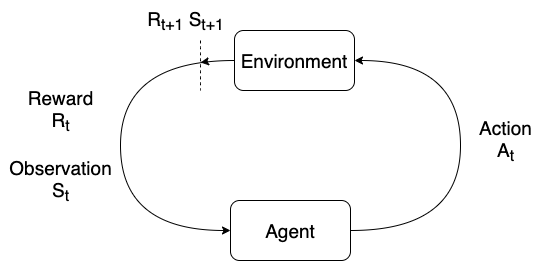
\includegraphics[width=0.75\textwidth]{images/agent_env_framework.png}
    \caption{Agent-environment interaction}
    \label{fig:lstm}
\end{figure}

To be precious, we formalize the environment as a Markov decision process (MDP) with state space $\mathcal{S}$, continuous action space $\mathcal{A}$ , the transition dynamics $p(s_{t+1} \mid s_t, a_t)$ and reward function $r(s_t, a_t)$. The reward function is hand-crafted and indicates whether the selected action in a certain state is considered "good" or "bad". The action selection process or rather the \textit{behaviour} of the agent is defined by a policy $\pi$, which is essentially a mapping from states to probabilities of actions being chosen $\pi: S \rightarrow P(A)$. But as we will exclusively calculate deterministic policies in this thesis, we define $\pi: S \rightarrow A$.
\par 
One of the major challenges arises from the nature of an MDP being a sequential decision problem. An action that seems to be mediocre in the present may result in an trajectory that produces better rewards in the long run and vice versa. It is therefore necessary to take future rewards into account. The discounted sum of future rewards is called the \textit{return} with a discounting factor $\gamma \in (0,1]$  \cite[p.55]{Sutton1998}:

\begin{equation}\label{eq:discountedReturn}
    G_t = R_{t+1} + \gamma R_{t+2} + \gamma^2 R_{t+3} + \dots  = \sum_{k=0}^\infty{\gamma^k R_{t+k+1}}
\end{equation}

By reshaping the above equation, we can discover the relationship between consecutive returns \cite[p.55]{Sutton1998}:
\begin{equation}\label{eq:successiveReturn}
    \begin{aligned}
    G_t &= R_{t+1} + \gamma R_{t+2} + \gamma^2 R_{t+3} + \gamma^3 R_{t+4} + \dots \\
    &= R_{t+1} + \gamma (R_{t+2} + \gamma R_{t+3} + \gamma^2 R_{t+4} + \dots)  \\
   & = R_{t+1} + \gamma G_{t+1}
    \end{aligned}
\end{equation}

The overall objective of an reinforcement learning agent is therefore to find an optimal policy that maximizes the return for a given starting state $s_0$. In order to do so, reinforcement learning algorithms try to estimate the expected return for any given state or state-action pair which is also called the \textit{value} or $Q$-value. The recursive relationship revealed in equation \ref{eq:successiveReturn} naturally applies to $Q$-values as well which is formally described by the \textit{Bellman equation} (for discrete policies):

\begin{equation}
    Q^\pi(s_t, a_t) = \EX_\pi[r(s_t, a_t) + \gamma Q^\pi(s_{t+1}, \pi(a_{t+1})]
\end{equation}


//TODMOB Tabular relationship